\section{Gates} \label{sec:gates}

Each gate is a row with 135 columns. As different custom gate has different complexity, for some complex gate 135 columns may only constraints one
operation while for other simple gate 135 columns may constraints several operations. The index of operation in a row is called slot.

Steps to use a custom gate:
\begin{itemize}
    \item Determine the type of gate;
    \item Find row and slot using gate type;
    \item Wire the operation parameters to cells found;
\end{itemize}

For the convenience of description, the trace tables in this paper only show one operation which is slot is 0.
\subsubsection{arithmetic\_base}

ArithmeticGate is a gate which can perform a weighted multiply-add, i.e.
\[ \text{res} = \text{cons\_0} \times \text{mul\_0} \times \text{mul\_1} + \text{cons\_1} \times \text{add}. \]

The structure of gate is shown in \figref{fig:arithmetic-gate}.

\begin{figure}[!ht]
    \centering
    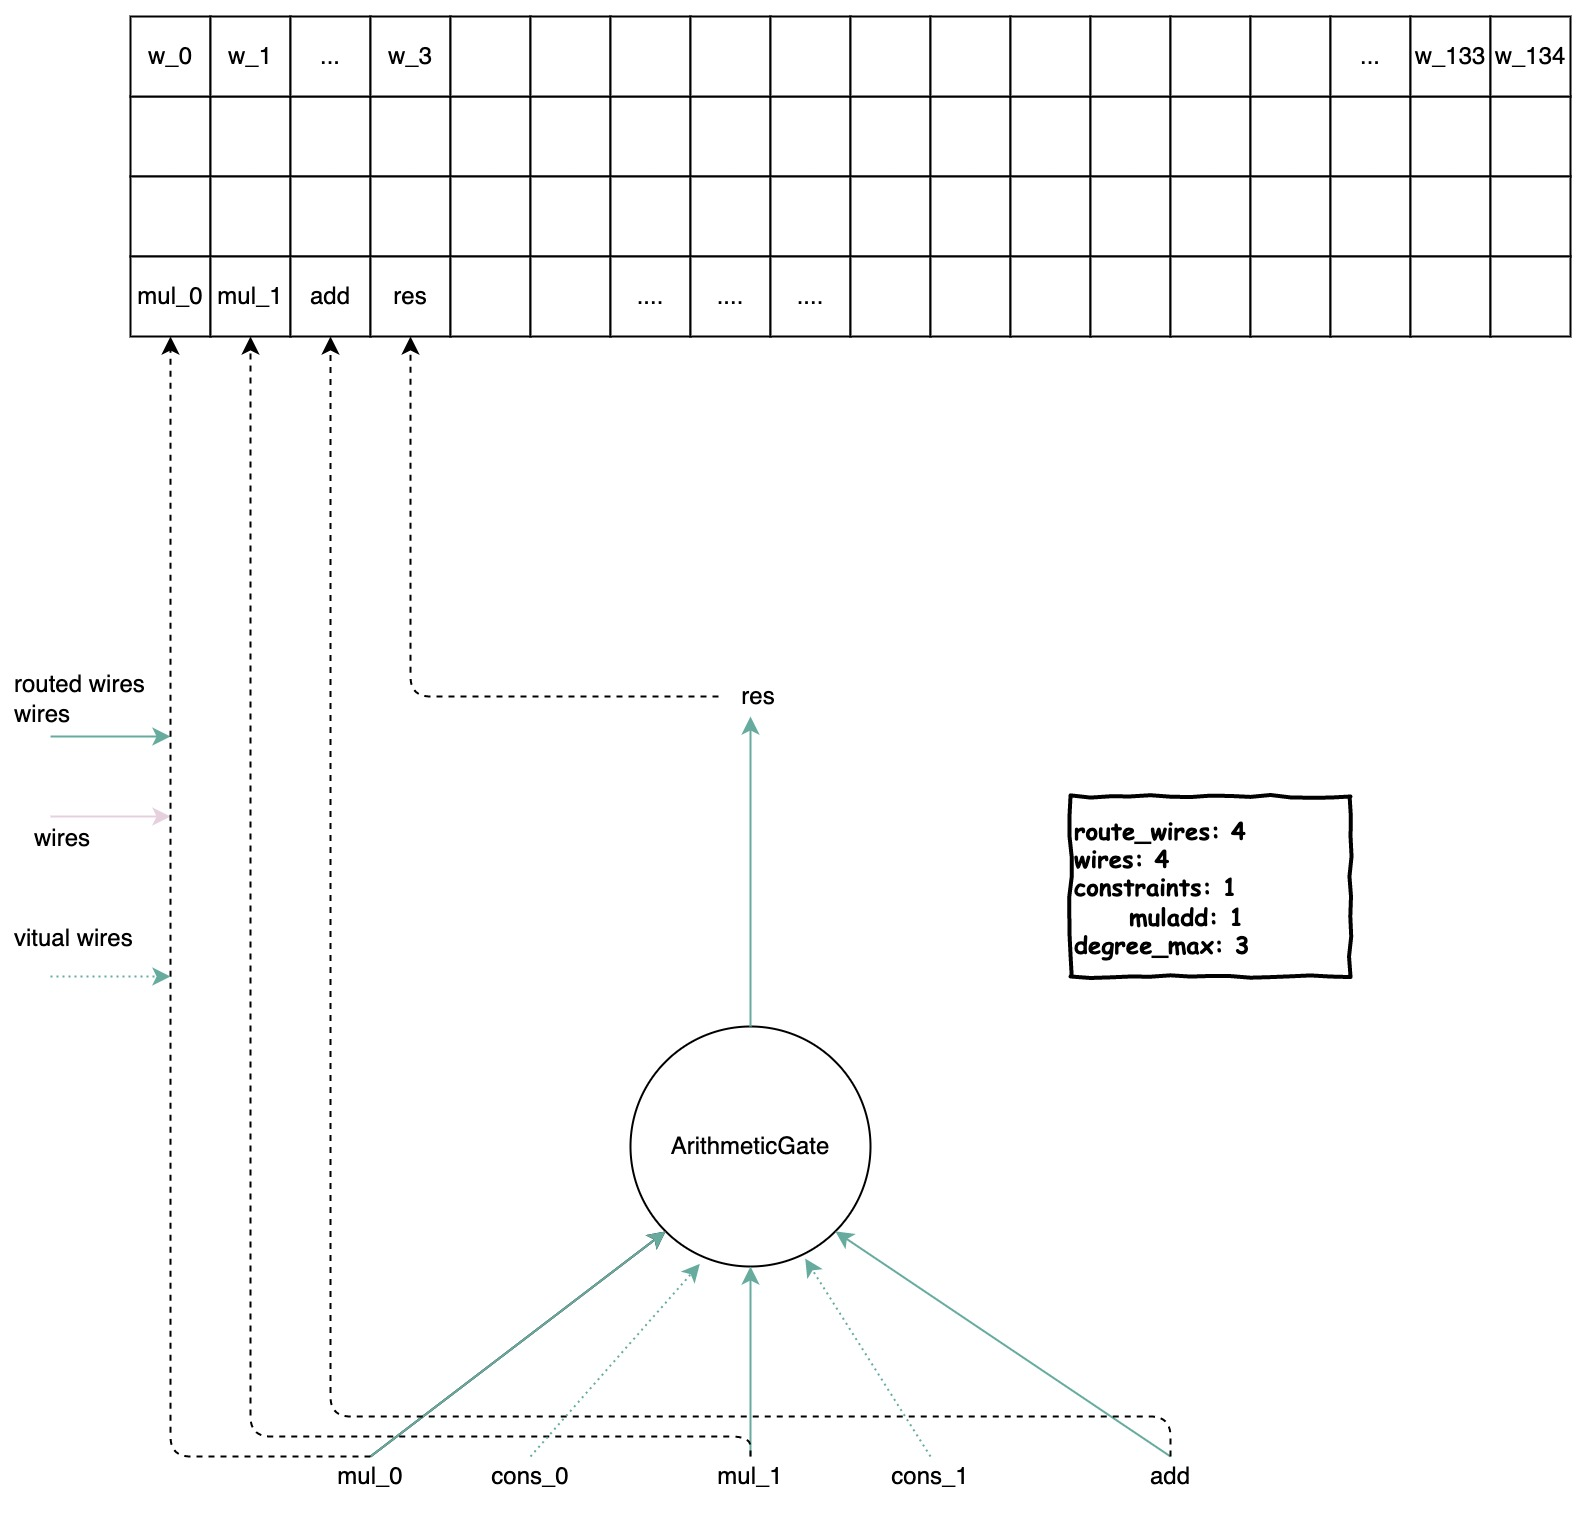
\includegraphics[width=0.8\textwidth]{gates/arithmetic_base.jpeg}
    \caption{ArithmeticGate}
    \label{fig:arithmetic-gate}
\end{figure}

There's only one constraint per operation, and degree is 3.

\subsection{arithmetic\_extension}

To understand the design principle of this Gate, we must first understand \href{https://en.wikipedia.org/wiki/Field_extension#Extension_field}{Field extension}. 


Taking Plonky2's GoldilocksField as an example, we give the extension field elements under quadratic, quadratic and quintuple expansions respectively:

\begin{figure}[!ht]
    \centering
    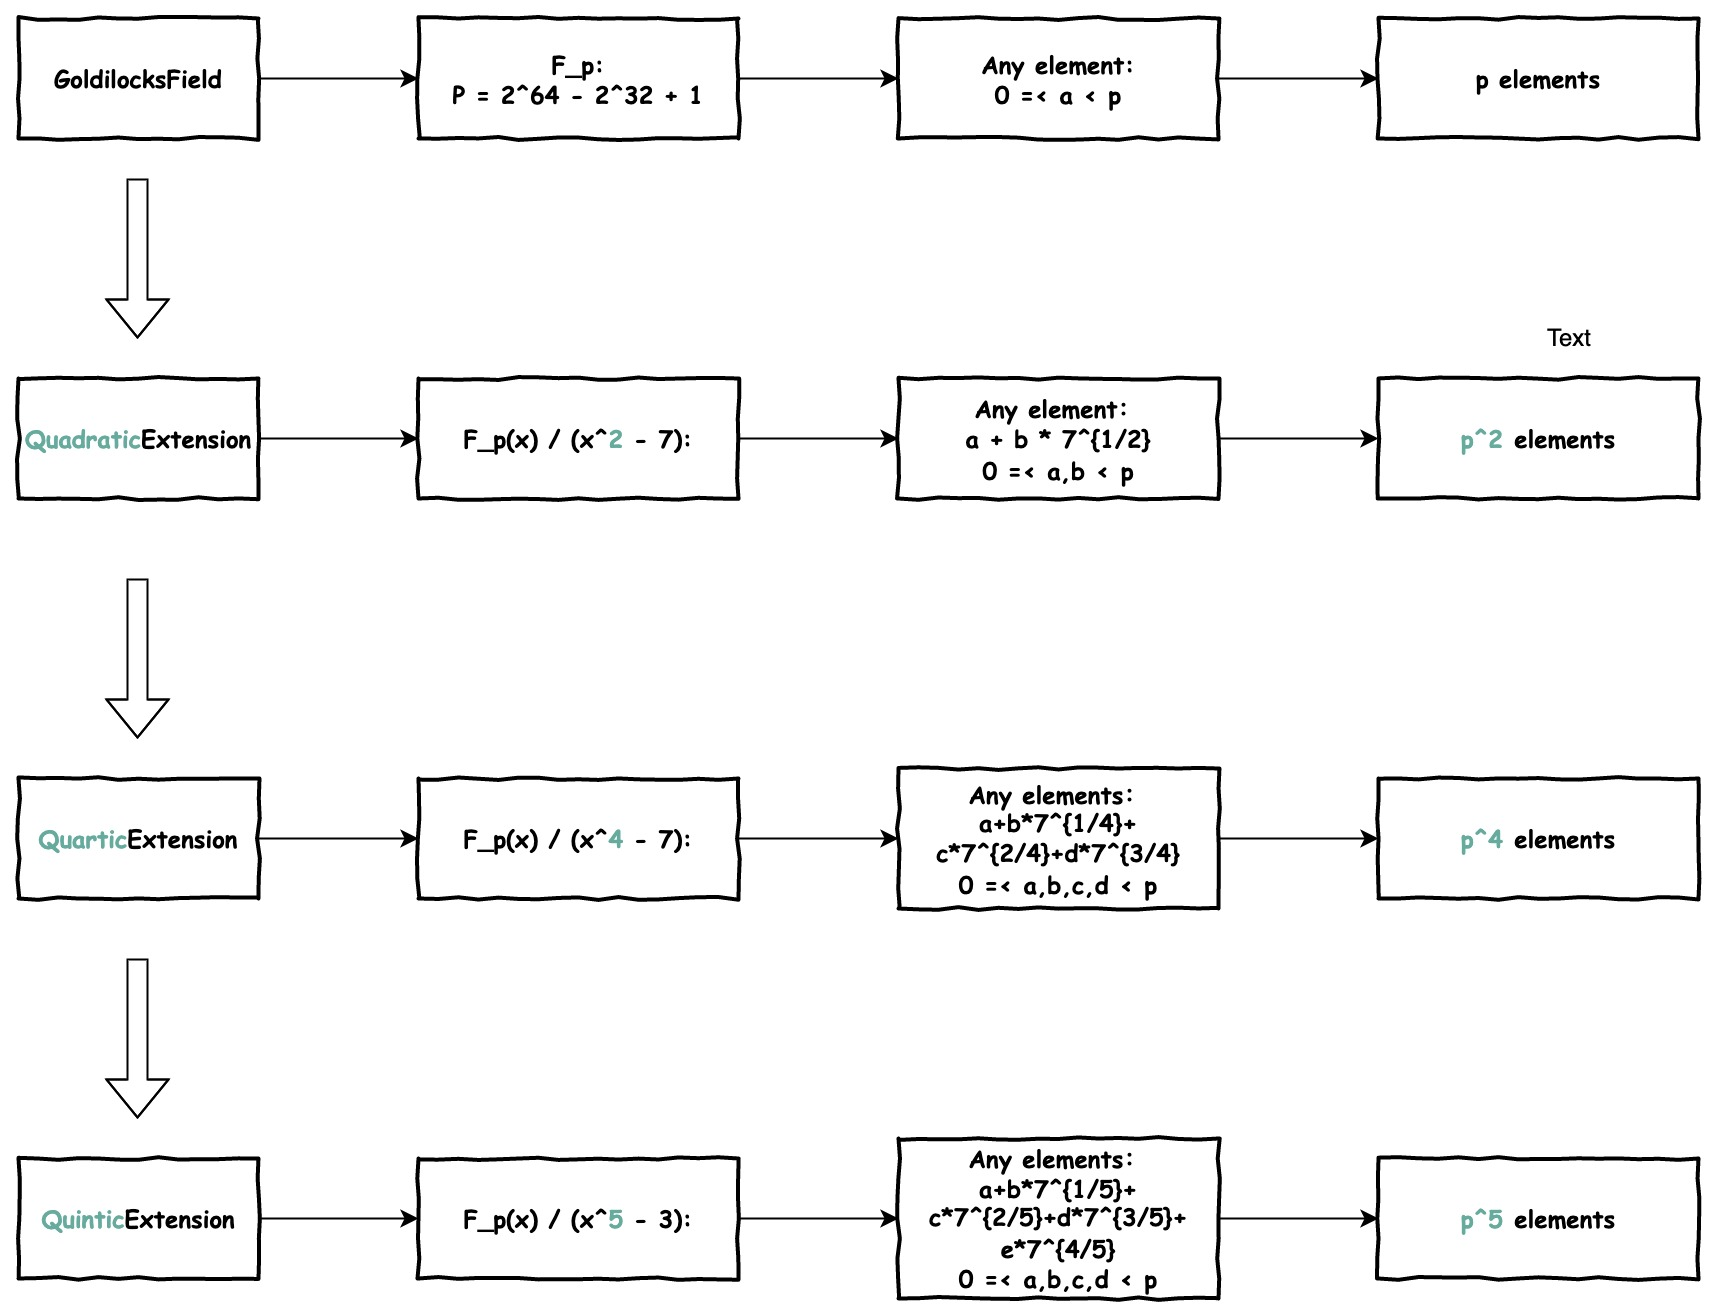
\includegraphics[width=0.8\textwidth]{gates/arthmetic_extension_ext.jpeg}
    \caption{GoldilocksField Extension}
    \label{fig:goldilocksfield-extension}
\end{figure}

It is easy to see that for QuadraticExtension Field, the elements on its domain take the form $a + b \sqrt{7}; a,b \subset F_p$, and a, b cannot both be 0.
It can be seen that on the quadratic extension domain, there are $p^2$ elements and the original domain is a subset of the quadratic extension domain.

ArithmeticExtensionGate is also a gate which can perform a weighted multiply-add, i.e.
\[res = cons\_0 * mul\_0 * mul\_1 + cons\_1 * add\]
The elements of the QuadraticExtension Field are represented in the form $[a, b]$, so the Gate design for arithmetic\_extension has the following form:

\begin{figure}[!ht]
    \centering
    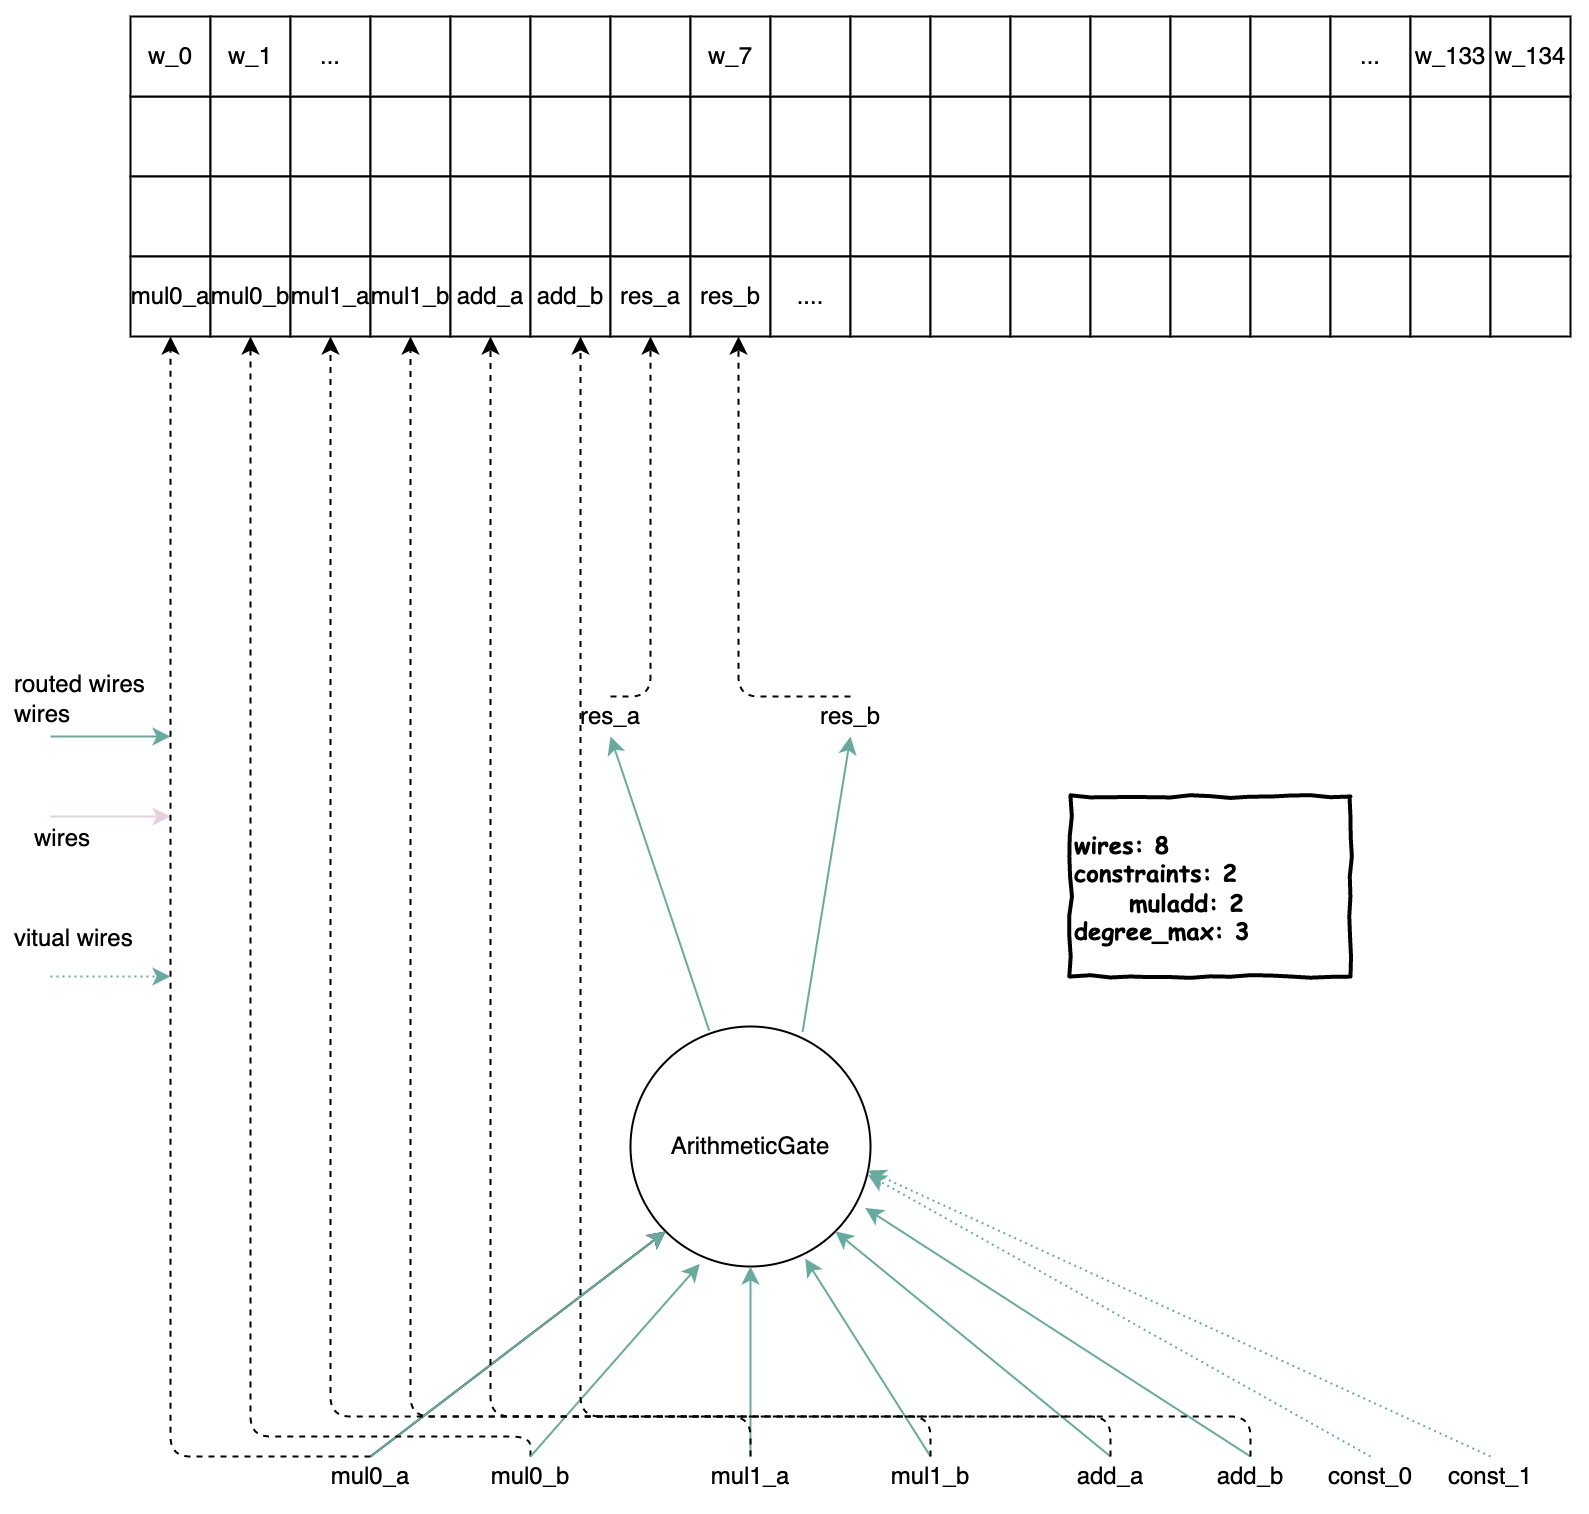
\includegraphics[width=0.8\textwidth]{gates/arthmetic_extension.jpeg}
    \caption{ArithmeticExtensionGate}
    \label{fig:arthmetic-extension}
\end{figure}
\subsubsection{base\_sum}

BaseSumGate is used to constrain the input to be composed of limbs which are arranged in little-endian. There are two kinds of constraints:

For each limb, limb is in range [0, base):
\[\sum_{i=0}^{base}(limb_i - i) = 0\]

Input is composed of limbs:
\[input = \sum_{i=0}^{n-1} limb_{n-1-i} * base^i\]

\begin{figure}[!ht]
    \centering
    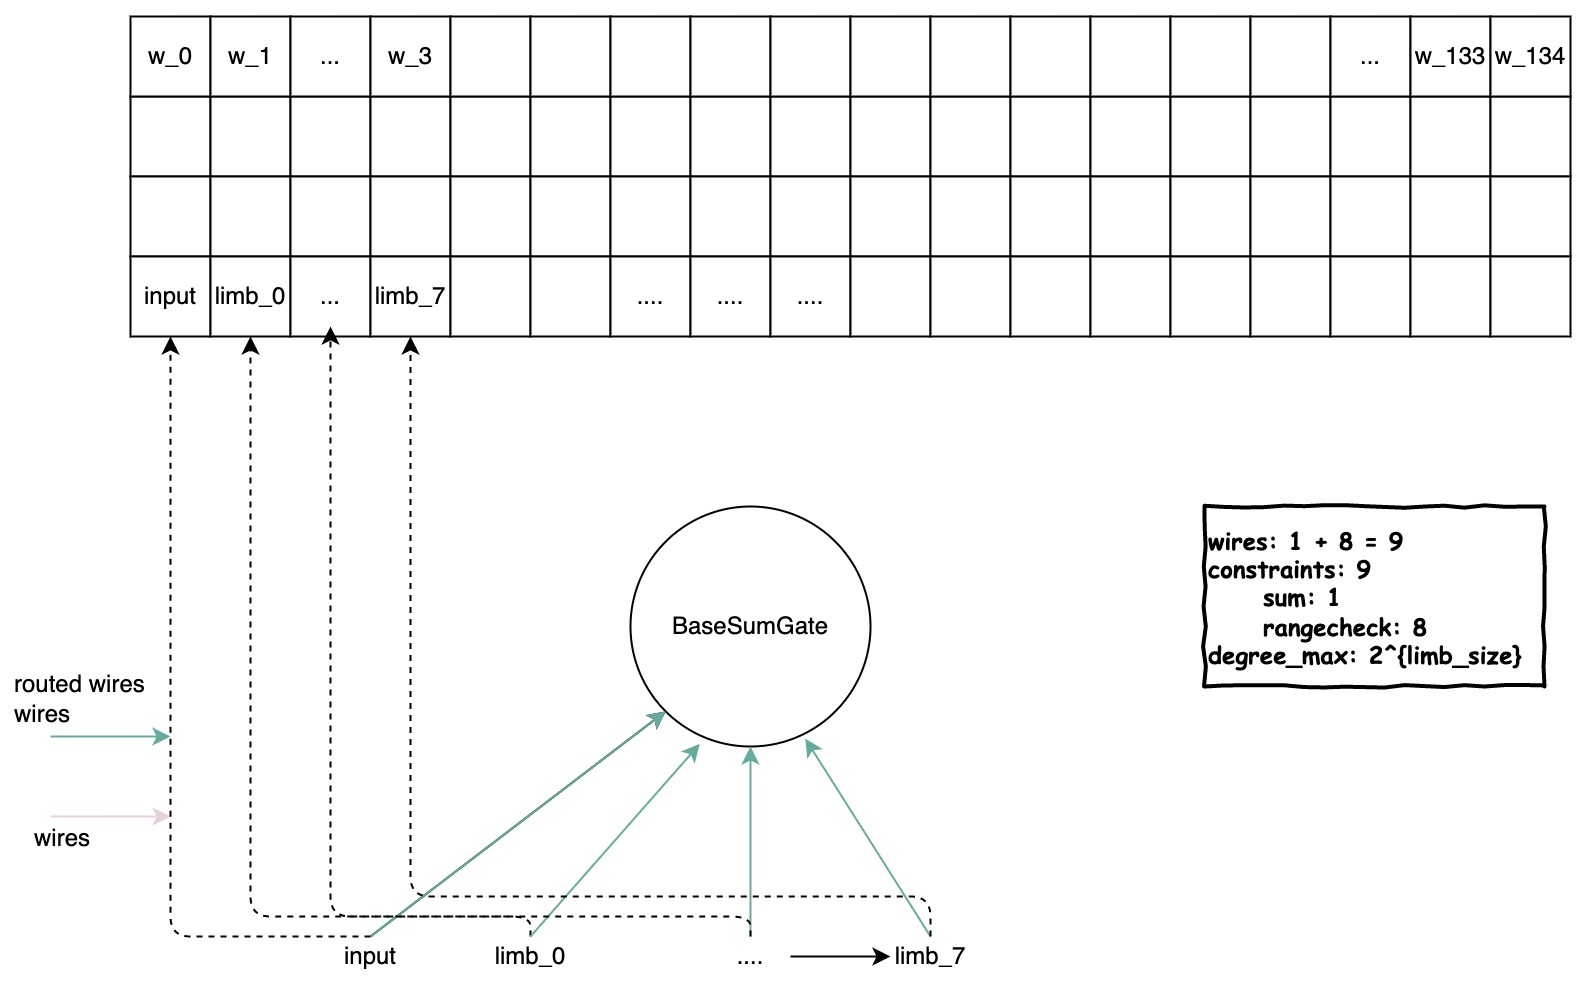
\includegraphics[width=0.8\textwidth]{gates/base_sum.jpeg}
    \caption{BaseSumGate}
    \label{fig:base-sum}
\end{figure}
\subsection{exponentiation}

ExponentiationGate is a gate for raising a value to a power. Trace table contains base, bits of the exponent, output, and intermediate value of the bits.

Take $A^{21} = A^{10101_b}$ for example to describe intermediate value, the bits are [1, 0, 1, 0, 1].

\begin{enumerate}
    \item Current bit=1, we start from 1, and times $A^{bit}$ we get $A$
    \item Current bit=0
    \begin{itemize}
        \item Square prev\_intermediate\_value $A^{1_b << 1} = A^{10_b}$
        \item Then times $A^{bit}$ we get $A^{10_b} * A^0 = A^{10_b}$
    \end{itemize}
    \item Current bit=1
    \begin{itemize}
        \item Square prev\_intermediate\_value $A^{10_b<<1} = A^{100_b}$
        \item Then times $A^{bit}$ we get $A^{100_b} * A = A^{101_b}$
    \end{itemize}
    \item Current bit=0
    \begin{itemize}
        \item Square prev\_intermediate\_value $A^{101_b << 1} = A^{1010_b}$
        \item Then times $A^{bit}$ we get $A^{1010_b} * 1 = A^{1010_b}$
    \end{itemize}
    \item Current bit=1
    \begin{itemize}
        \item Square prev\_intermediate\_value $A^{1010_b << 1} = A^{10100_b}$
        \item Then times $A^{bit}$ we get $A^{10100_b} * A = A^{10101_b}$
    \end{itemize}
\end{enumerate}

And we get the last intermediate value $A^{10101_b}$ which should be equal to the output.

Let's take another example of a specific number $2^13 = 2^{1101_b}$, and have a look at the trace cell:
\begin{center}
    \begin{tabular}{ |c|c|c|c|c|c|c|c|c|c| }
        \hline
        base & b\_0 & b\_1 & b\_2 & b\_3 & output & inter\_0 & inter\_1 & inter\_2 & inter\_3 \\
        \hline
        2 & 1 & 0 & 1 & 1 & 8192 & 2 & 8 & 64 & 8192 \\
        \hline
    \end{tabular}
\end{center}

The structure of Gate is shown in the figure:
\begin{figure}[!h]
    \centering
    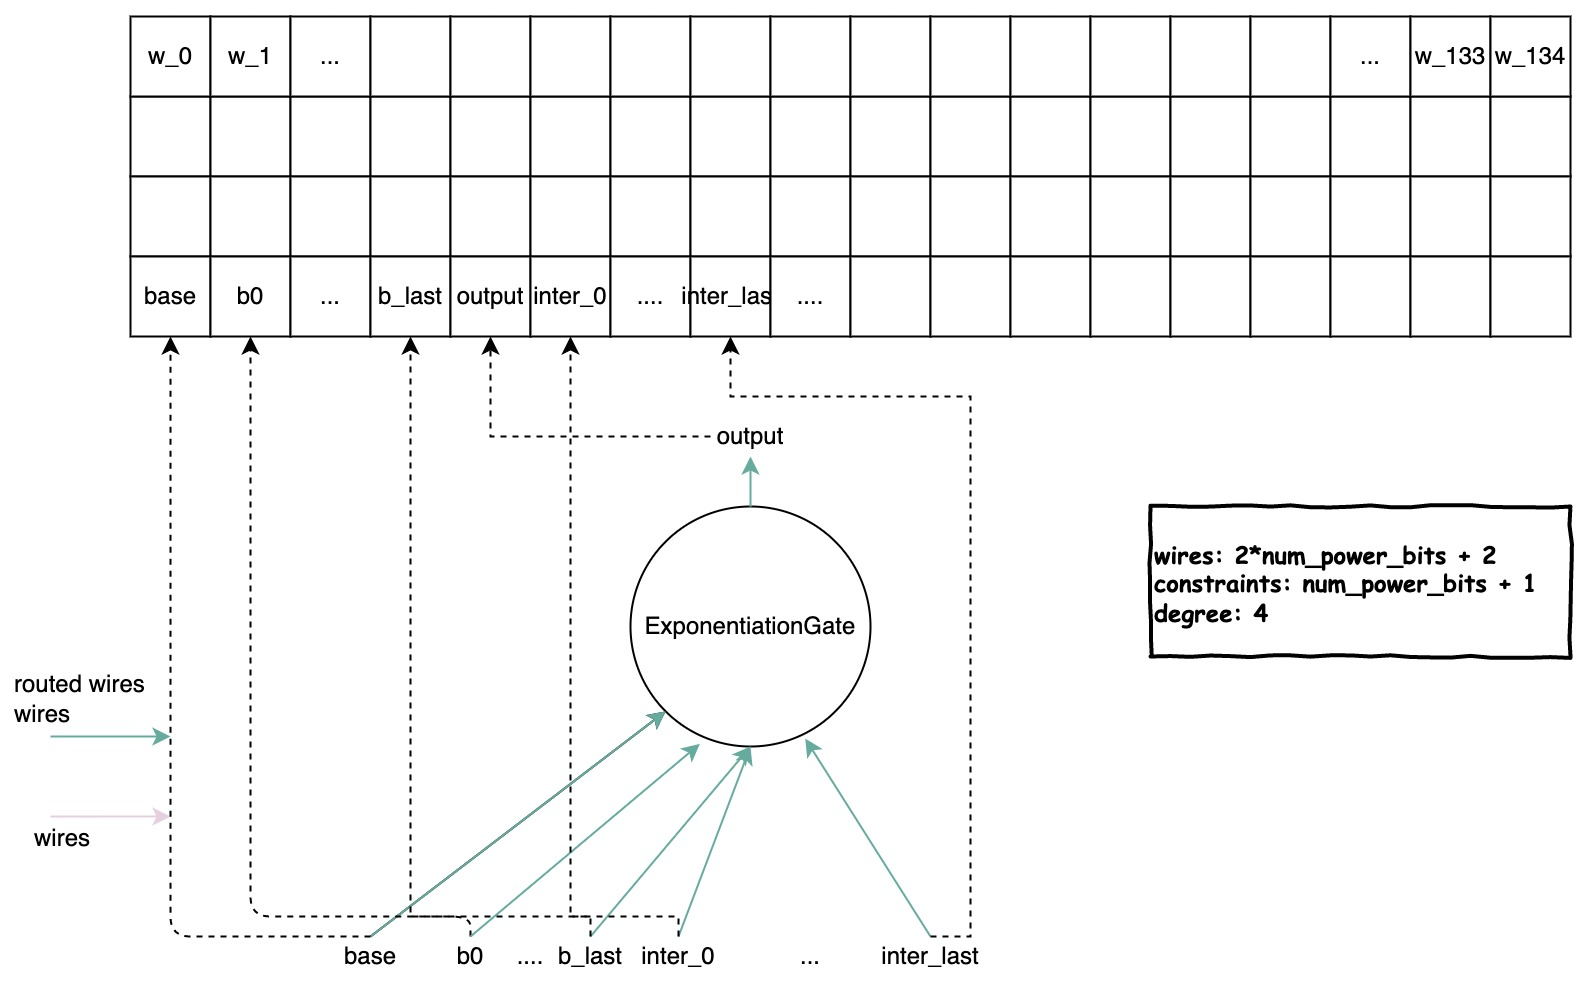
\includegraphics[width=0.8\textwidth]{gates/exponentiation.jpeg}
    \caption{ExponentiationGate}
    \label{fig:exponetiation-gate}
\end{figure}
